\chapter{Storage: Architetture e Servizi}

\section{Evoluzione del Mezzo di Memorizzazione}
Lo storage rappresenta il secondo pilastro fondamentale di un datacenter, il luogo dove i dati persistono alla perdita di alimentazione (persistenza). La regola assoluta dello storage è una sola: \textbf{perdere i dati è il peccato imperdonabile}.

\subsection{Dal Nastro Magnetico all'HDD e all'SSD NVMe}
Storicamente, i primi datacenter utilizzavano \textbf{Nastri Magnetici (Tape)}: cartucce robotiche lente ma dalla capacità e densità enormi. Il nastro costringe ad un accesso sequenziale ai dati (non si può saltare alla fine senza "srotolare" tutto), ma è ancora oggi impiegato per il cold storage e i backup offline impenetrabili ai ransomware (Air-gap).

\begin{figure}[H]
    \centering
    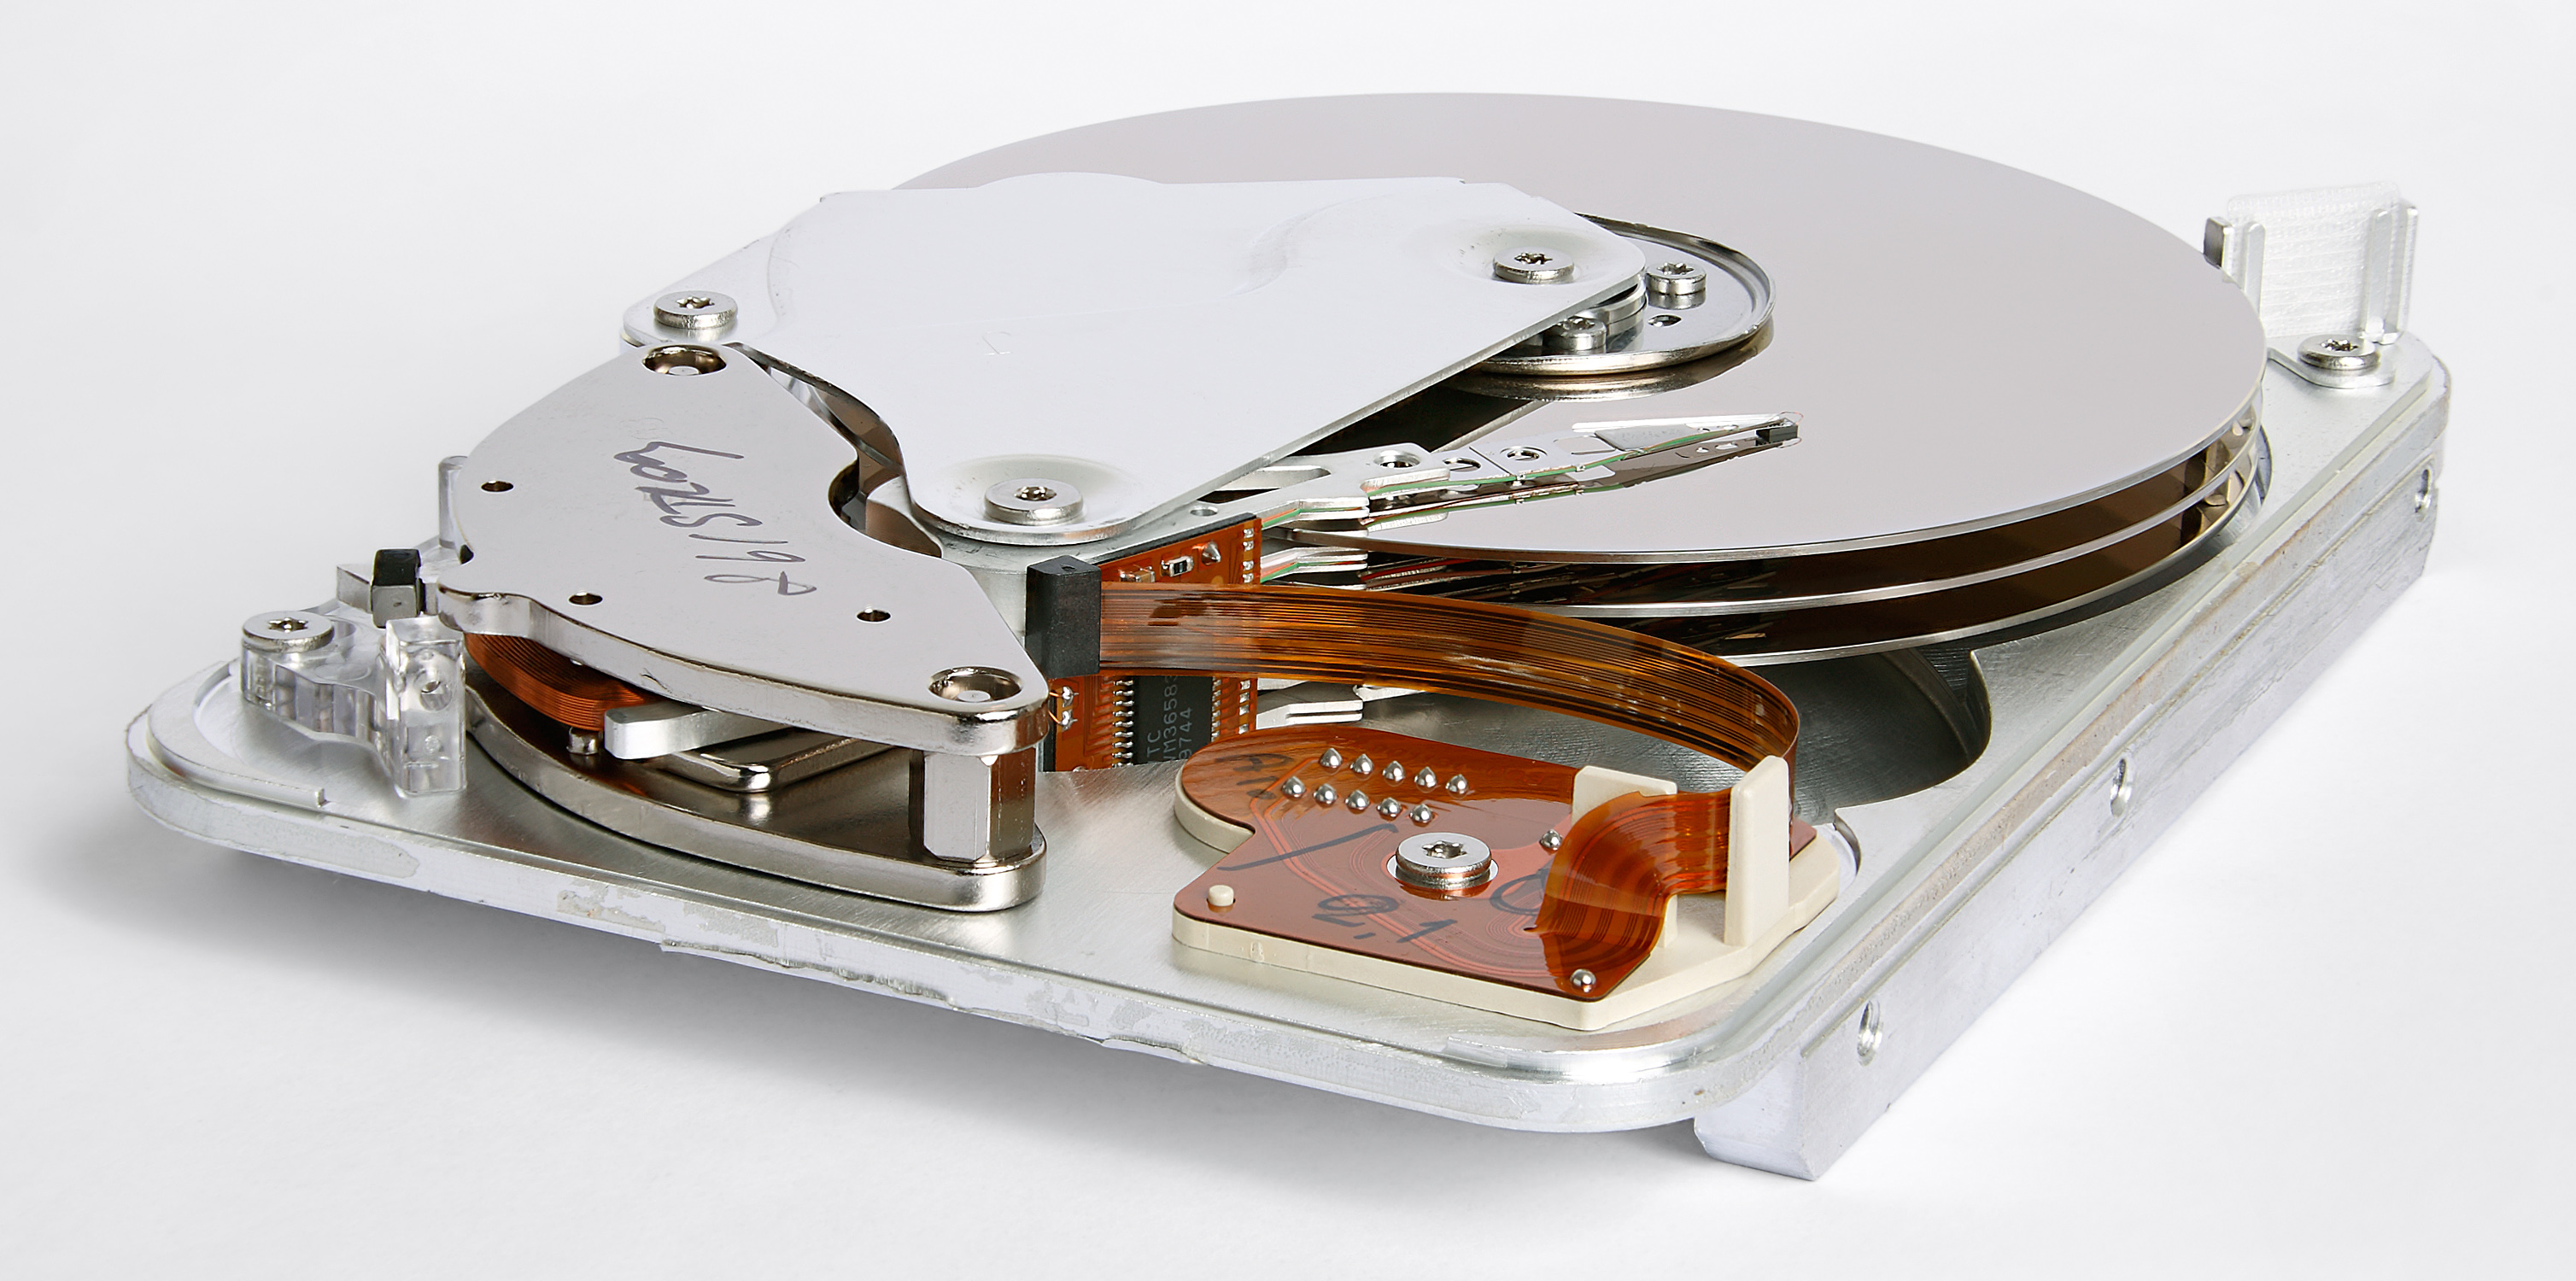
\includegraphics[width=0.6\textwidth]{images/hdd_inner.jpg}
    \caption{Interno di un Hard Disk Drive magnetico meccanico tradizionale.}
\end{figure}
Successivamente, si è passati agli \textbf{HDD (Hard Disk Drive)}, che offrono accesso casuale ai dati. Tuttavia, essi sono limitati da vincoli meccanici (rotazione dei piatti, tempo di \textit{seek} della testina), con latenze invalicabili di circa 3-5 ms. Le configurazioni storiche per i server usavano interfacce complesse in cascata (es. \textbf{SCSI}), oggi sostituite da protocolli SAS o SATA. Attualmente gli HDD sono relegati quasi esclusivamente all'archiviazione di massa a basso costo.

La transizione verso gli \textbf{SSD (Solid State Drive)} ha abbattuto la latenza a poche centinaia di microsecondi. Tuttavia, l'uso dei vecchi controller SATA si è rivelato rapidamente un collo di bottiglia. La rivoluzione successiva è stata l'introduzione dello standard \textbf{NVMe (Non-Volatile Memory Express)}, un protocollo che collega direttamente la memoria flash al bus \textbf{PCIe}, portando la latenza a $\sim$5-20 $\mu$s e il throughput a decine di GB/s.

\begin{tipbox}[Gerarchia della Memoria Moderna]
Con NVMe, il divario prestazionale tra DRAM (nanosecondi) e storage permanente (microsecondi) si è ridotto da 6 a soli 2 ordini di grandezza, permettendo architetture software impensabili prima, come database (es. RocksDB) che operano direttamente su storage senza pesanti strati di caching in RAM.
\end{tipbox}

\subsection{Celle NAND e Asimmetria}
A differenza della DRAM, la memoria NAND Flash presenta un'asimmetria intrinseca: le operazioni di lettura sono veloci, mentre le scritture richiedono un ciclo PE (Program/Erase) molto più lento. La densità dei bit per cella determina il tipo di SSD:
\begin{itemize}
    \item \textbf{SLC (Single-Level Cell):} 1 bit, altissima resistenza (100k cicli PE), altissimo costo.
    \item \textbf{MLC, TLC, QLC:} rispettivamente 2, 3 e 4 bit per cella. Costi decrescenti ma resistenza (endurance) e prestazioni in scrittura in rapido calo.
\end{itemize}

\subsection{Misure di Performance: IOPS, Latenza e Bandwidth}
Latenza e Bandwidth (throughput) da sole non sono sufficienti per caratterizzare le prestazioni di uno storage, poiché dipendono fortemente dal pattern di accesso (sequenziale o casuale). 
Una metrica fondamentale è l'\textbf{IOPS} (Input/Output Operations Per Second), ovvero il numero di operazioni di I/O completate in un secondo.
\begin{itemize}
    \item \textbf{Analogia del supermercato:} Gli IOPS rappresentano i clienti serviti al secondo, la latenza è il tempo impiegato in cassa per ogni cliente, e il parallelismo (le code) sono le casse aperte.
    \item La relazione base per una singola coda è: $\text{IOPS} \approx \frac{1}{\text{latenza}}$.
    \item Grazie alla natura asincrona dello storage, protocolli come NVMe (che supportano fino a 64.000 code parallele) permettono di scalare immensamente il throughput elaborando molte richieste simultaneamente.
\end{itemize}

\section{Aggregazione e Protezione: Il RAID}
Un singolo disco è un single point of failure inaccettabile. Si utilizza quindi il \textbf{RAID} (Redundant Array of Inexpensive Disks):
\begin{itemize}
    \item \textbf{RAID 0 (Striping):} Nessuna ridondanza, altissime prestazioni, rischio massimo.
    \item \textbf{RAID 1 (Mirroring):} Copia identica, perde il 50\% dello spazio.
    \item \textbf{RAID 5:} Ridondanza calcolata tramite funzione logica \textbf{XOR}. Tolleranza alla rottura di 1 solo disco. Se un secondo disco si rompe durante la fase di \textit{rebuild}, si perdono tutti i dati.
    \item \textbf{RAID 6:} Usa doppia parità, permettendo il fallimento simultaneo di \textbf{2 dischi}. È lo standard de facto nei datacenter odierni per via delle grandi capacità dei drive e dei lunghi tempi di rebuild.
\end{itemize}

\section{Architetture di Storage nel Datacenter}

\subsection{SAN (Storage Area Network)}
La SAN centralizza lo storage separandolo dai server, comunicando a livello di blocco (espone dischi grezzi, non file). I protocolli dominanti per questo fabric sono:
\begin{itemize}
    \item \textbf{Fibre Channel (FC):} Una rete fisicamente e logicamente separata dall'Ethernet standard. Richiede schede dedicate sui server, dette \textbf{HBA (Host Bus Adapter)}, e switch FC dedicati. Identifica i nodi non tramite MAC address, ma tramite indirizzi a 64 bit chiamati \textbf{WWN (World Wide Name)}.
    \item \textbf{iSCSI:} Alternativa economica che trasporta i comandi SCSI all'interno di normali pacchetti TCP/IP su rete Ethernet. Funziona tramite un'architettura client-server: il server host agisce da \textbf{iSCSI Initiator} (che richiede i blocchi), mentre lo storage array è l'\textbf{iSCSI Target} (che li fornisce). I nodi sono identificati tramite stringhe \textbf{IQN}.
    \item \textbf{FCoE (Fibre Channel over Ethernet):} Il tentativo di unificare le due reti. Incapsula i frame FC direttamente dentro l'Ethernet standard, eliminando la necessità di stendere cavi in fibra separati e riducendo il numero di switch, ma mantenendo il protocollo FC senza l'overhead del TCP/IP.
\end{itemize}

\begin{tipbox}[Sicurezza SAN: Zoning e Masking]
Per evitare che un server formatti per errore il disco (o intercetti i dati) di un altro server, si usano due barriere:
\begin{enumerate}
    \item \textbf{Zoning (Lato Rete):} Applicato sugli switch, crea zone hardware chiuse. Simile al concetto di VLAN nell'Ethernet, impedisce a due HBA che non sono nella stessa zona di comunicare o "vedersi" a vicenda.
    \item \textbf{LUN Masking (Lato Storage):} Lo storage array autorizza l'accesso a un disco logico (\textbf{LUN, Logical Unit Number}) esclusivamente allo specifico indirizzo WWN (per FC) o IQN (per iSCSI) del server proprietario.
\end{enumerate}
\end{tipbox}

\subsection{NAS (Network Attached Storage)}
Il NAS opera a un livello di astrazione più alto, connesso tramite rete Ethernet standard (protocolli NFS o SMB).
\begin{itemize}
    \item \textbf{Astrazione:} Espone un File System logico (\textit{file e directory}).
    \item \textbf{Limiti:} Maggiore latenza e impossibilità di usare la tecnica del \textit{memory mapping} in rete.
    \item \textbf{Casi d'uso:} File sharing, backup, documenti aziendali.
\end{itemize}

\subsection{Object Storage}
Sviluppato per gestire scalabilità a livello di Exabyte (es. Amazon S3). Abbandona cartelle e blocchi, utilizzando \textbf{oggetti} piatti allocati in \textit{bucket} e interrogabili tramite API REST.
Per garantire la scalabilità e distribuire i dati senza un collo di bottiglia centrale, utilizza algoritmi di routing come il \textbf{Consistent Hashing}. Ideale per dati statici e massivi, come dataset di Machine Learning o archivi medici.

\subsection{HCI (Hyper-Converged Infrastructure)}
Per decenni il mercato datacenter è stato dominato da grandi vendor che fornivano SAN e NAS hardware proprietari (es. i famosi array \textbf{EMC Symmetrix} o i \textbf{Filer NetApp}), apparati costosissimi e dal difficile scaling orizzontale. 
Per abbattere i costi e scalare linearmente, si è passati all'\textbf{HCI}, che trasforma lo storage SAN centralizzato in un approccio distribuito (*Scale-out*). Ogni server (nodo commodity x86) contiene CPU, RAM e dischi NVMe locali. Un livello software (Software-Defined Storage) raggruppa tutti i dischi locali di tutti i nodi e li presenta all'hypervisor come un'unica grande SAN virtuale condivisa.
\begin{tipbox}[Vantaggio dell'HCI]
\textbf{Data Locality:} Il software tenta sempre di scrivere/leggere i dati di una VM nel disco fisicamente residente nello stesso server che la esegue, azzerando il traffico di rete Nord-Sud e sfruttando al massimo la banda PCIe locale.
\end{tipbox}

\subsection{Storage per l'AI: Vector Database}
L'emergere dell'Intelligenza Artificiale generativa ha richiesto nuovi paradigmi di memorizzazione. La ricerca testuale classica era puramente \textit{sintattica} (come nel modello \textit{bag of words}), mentre i modelli neurali operano sulla \textit{semantica}.
\begin{itemize}
    \item \textbf{Embeddings:} Le reti neurali (LLM) trasformano testi, immagini o audio in vettori densi ad altissima dimensionalità (es. 3000 dimensioni). Questi vettori, chiamati \textit{embedding}, rappresentano il reale significato del dato in base al contesto (es. distinguono "Python" come linguaggio da "Python" come serpente).
    \item \textbf{Vector Database:} Sono una nuova generazione di database NoSQL progettati specificamente per immagazzinare e indicizzare questi enormi vettori. Per rispondere a una query, vettorializzano la domanda dell'utente e cercano i documenti semantici più simili calcolando la \textbf{distanza coseno} nello spazio vettoriale.
\end{itemize}
\begin{tipbox}[RAG: Retrieval-Augmented Generation]
I Vector Database sono il motore dell'architettura \textbf{RAG}, tecnica essenziale per limitare le "allucinazioni" delle AI. Prima di rispondere a un prompt, il sistema interroga il vector database, recupera i documenti aziendali realmente pertinenti, li inietta nel prompt e obbliga il LLM a formulare la risposta basandosi unicamente su quei fatti verificati.
\end{tipbox}

\section{Servizi Avanzati e Resilienza}

\subsection{Snapshot, Thin Provisioning e Replica}
\begin{itemize}
    \item \textbf{Thin Provisioning:} Permette di allocare logicamente più spazio agli utenti rispetto a quanto fisicamente presente nello storage, basandosi sul principio che raramente lo spazio allocato viene subito riempito (\textit{Overcommitment}). Il rischio intrinseco è esaurire fisicamente lo spazio se tutti gli utenti scrivono contemporaneamente, causando un blocco sistemico dei dischi.
    \item \textbf{Snapshot vs Clone:} La \textit{Snapshot} è una fotografia istantanea del volume che occupa inizialmente zero spazio aggiuntivo. Sfrutta il meccanismo del \textbf{Copy-on-Write (COW)}: congela i blocchi originali e alloca nuovi blocchi solo per le successive scritture. Se i dati originali si rompono, la snapshot è inservibile perché basata su puntatori condivisi. Un \textbf{Clone}, invece, è una copia fisica completa bit-a-bit (che impiega tempo e spazio) ed è totalmente indipendente.
    \item \textbf{Replica Sincrona/Asincrona:} Indispensabile per il Disaster Recovery. Nel caso di siti geografici vicini (max 300 km o 15ms di latenza round-trip), è possibile realizzare \textbf{Metro Cluster} con replica sincrona active-active.
\end{itemize}

\subsection{Backup vs Replica}
La \textbf{replica} è una copia speculare in tempo reale: protegge dai guasti hardware, ma propaga istantaneamente cancellazioni umane o attacchi ransomware. Il \textbf{backup} è un salvataggio point-in-time e sconnesso (offline) che permette il recupero.

Nel dimensionamento di un sistema di continuità aziendale due metriche sono fondamentali:
\begin{itemize}
    \item \textbf{RPO (Recovery Point Objective):} Quantità di dati che l'azienda è disposta a perdere (frequenza dei backup).
    \item \textbf{RTO (Recovery Time Objective):} Tempo massimo tollerabile per il ripristino dell'infrastruttura.
\end{itemize}

\begin{warningbox}[GDPR e Data Breach]
Secondo il GDPR, un \textit{data breach} non è solo il furto dei dati (perdita di \textit{confidenzialità}), ma include anche la perdita di \textit{integrità} (dati corrotti) e di \textbf{disponibilità} (dati integri ma non accessibili, ad esempio durante un attacco ransomware che cifra l'unico storage primario).
\end{warningbox}
